%
%  Microssa-Documentation.tex
%
%  Copyright (C) 2015 Michael Dinolfo
%
%  This program is free software: you can redistribute it and/or modify
%  it under the terms of the GNU General Public License as published by
%  the Free Software Foundation, either version 3 of the License, or
%  (at your option) any later version.
%
%  This program is distributed in the hope that it will be useful,
%  but WITHOUT ANY WARRANTY; without even the implied warranty of
%  MERCHANTABILITY or FITNESS FOR A PARTICULAR PURPOSE.  See the
%  GNU General Public License for more details.
%
%  You should have received a copy of the GNU General Public License
%  along with this program.  If not, see <http://www.gnu.org/licenses/>.
%

\documentclass[Letter]{article}
\usepackage[T1]{fontenc}
\usepackage{lmodern}
\usepackage[english]{babel}
\usepackage{fontspec}
\usepackage{graphicx}
\setmainfont{DejaVu Sans}
\hyphenpenalty=500

\title{Microssa Documentation}
\date{Michael Dinolfo <mike@dinolfo.us>}
\author{Version 1.4}

\begin{document}

\pagenumbering{gobble}
\maketitle
\newpage
\tableofcontents
\newpage
\pagenumbering{arabic}

\section{Overview}

Microssa is a free matching engine written in Java which includes a FIX engine and database integration.


\subsection{Mission}

This software was created with the following goals:

\begin{itemize}
    \item Free: This software's license (GPL, "copyleft")
    gives rights to the users while ensuring copies and derivatives
    remain under such a license.  Required dependencies must
    be under permissive licenses.
    \item Agnostic: This matching engine does not care
    what it is trading.  It can be things real or virtual, securities,
    currency, or goods.
\end{itemize}

However, within the terms the GPL license, you are free to use this
software and modify it for any purpose you desire.  See the file
\texttt{LICENSE} in the root project directory for the complete details.


\subsection{Examples of Use}

This software was created with the following use cases in mind:

\begin{itemize}
    \item Bitcoin or other cryptocurrency exchange
    \item Market in a simulated environment, such as a video game
    \item Virtual stock exchange used to develop a trading algorithm
\end{itemize}

Currently, Microssa would be a poor choice for:

\begin{itemize}
    \item Production stock exchange or ECN: this software lacks
    compliance checks and 3rd party reporting.
    \item High speed trading: this software is currently not optimized
    for this purpose.
\end{itemize}


\subsection{Non-Permissive Licenses or Customizations}

Contact Michael Dinolfo if you or your organization would like a release
of Microssa under a different license, or are interested in the
development of custom logic that suits your needs.

\subsection{Getting Started}

\subsubsection{Dependencies}

\begin{description}
    \item[OpenJDK 8] Required to build.  Building may also work with Sun's
    version 8 JDK.
    \item[Quickfix/J] Required to build. Microssa was last tested with the
    all jar version 1.6.4 but may work with other configurations. This jar
    is the primary API called by the FIXInterface class. Quickfix/J has its
    own dependencies which are required for Microssa to run:
    \begin{description}
        \item[mina] tested with version 2.0.17
        \item[slf4j api] tested with version 1.7.25
        \item[slf4j jdk] tested with version 1.7.25
    \end{description}
    \item[make] Recommended.  Allows the project to be built with
    relative ease.  See the following two subsections for the difference.
    \item[expect] Recommended.  Allows use of the test suite scripts
    located in the \texttt{test} folder.
    \item[texlive] Optional.  Allows rebuilding of this document.
    \item[DejaVu Sans font] Optional.  Allows rebuilding of this document.
    \item[LibreOffice] Optional.  Allows modifying of diagram at the end
    of this document.
    \item[MySQL] Optional.  A database to read incoming
    orders and store trade reports.
    \item[Connector/J] Optional. The API Microssa will use to communicate
    with a MySQL database.
\end{description}

\subsubsection{Building the JAR with make}

Go to the home directory of the Microssa project.  Run the following to
build the project:
\begin{verbatim}
make
\end{verbatim}

This will compile the java files in \texttt{src/Microssa}, build a
jar file, and place the jar in the \texttt{bin} folder.

\subsubsection{Building the JAR without make}

Go to the home directory of the Microssa project.  Run the following to
build the project:
\begin{verbatim}
cd src/Microssa
javac *.java
cd ..
jar cfm Microssa.jar MANIFEST.MF Microssa/
mv Microssa.jar ../bin
\end{verbatim}

\subsubsection{Configuration}
The file \texttt{Microssa.cfg} in the \texttt{bin} folder contains
settings to modify the log file name, ports opened, and matching engine
logic.  Comments within the file explain each available option and
its usage.

\subsubsection{Starting Microssa}

Change into the \texttt{bin} folder and run the shell script
\texttt{./start-microssa.sh}.  Optionally, you can start with
\texttt{java -jar Microssa.jar}.  Starting will not return the prompt, nor
anything to it unless there is an exception. Rather, the file
\texttt{Microssa.log} shows the matching engine's actions.  See the
\texttt{Socket Interfaces} section of this document on how to interact
with the matching engine.

\subsection{Financial Terminology}

The source code and documentation of this project contain a lot
of financial language.  This section is intended to define and clarify
many of those terms.

\subsubsection{Order}

An order is a party's willingness to buy or sell some amount of a
real or virtual object at a specified price.  Other attributes of an
order serve as identifiers or special instructions.  See the section
on the \texttt{Order Object} for more details.

\subsubsection{Symbol}

Text identifier for the object that the order is trying to buy or sell.
Examples include specific stocks (AAPL for Apple), options, currency
 (USD v GBP), bonds, or Bitcoins (BTC/BTX).

\subsubsection{Match, Execution, Fill}

Two orders can match when:

\begin{itemize}
    \item One is buying.
    \item One is selling.
    \item They are for the same Symbol.
    \item Their prices are compatible: either they have the same price,
    or the buyer is willing to bid more than what the seller is offering.
\end{itemize}

Each order then gets and execution, or fill.  An order is said to
be fully filled or completed if the match, or the sum of all of its
matches, is equal to its entire Quantity.

Other conditions can affect match eligibility such as currency,
settlement date, and minimum fill quantity.

\subsubsection{Time in Force}

Specifies the lifetime of an order.  The two most common options are:

\begin{itemize}
    \item Immediate or Cancel: IOC orders enter a matching engine and
    attempt to execute immediately.  These orders then expire, if not
    fully filled.
    \item Good for Day: DAY/GFD orders enter a matching engine and
    attempt to execute immediately.  These orders then become passive
    orders if not fully filled.  They can be filled against orders that
    arrive at a later time.  DAY/GFD orders expire at the end of the
    trading day.
\end{itemize}

\subsubsection{Book, Passive, Aggressive}

A book is a list of passive, or resting, orders.  These orders had
insufficient matches to fully fill them at the time they entered the book.
An aggressive order is a new/amended order that enters a matching engine
and matches before being written to the book.  A match always consists
of one passive order and one aggressive order.  An IOC order can only
be an aggressive order, but a DAY/GFD order can fill either role.

\subsubsection{Market, Exchange, ECN}

Locations where orders are sent to be matched.  Each typically consists
of a matching engine, interfaces such as FIX engines or message queues,
market data feeds, and execution feeds.

\subsubsection{Matching Engine}

The part of a market, exchange, or ECN that matches the orders.
Microssa is a matching engine.

\subsubsection{Interface, FIX Engine, Message Queue}

These connections electronically link the matching engine to the outside
world.  They allow parties to send and manage orders to a matching
engine, and to for the engine to notify the parties on the state of
their orders.

\subsubsection{Market Data}
The display of prices and quantities for passive orders.  This
information is used by traders help them determine what kind of order
they want to send to the market.

\subsubsection{Execution Feed or Ticker}
The display of trades that occurred on the matching engine.
Traditionally shows the object traded, the price, and the quantity,
but one or both parties may not be shown to protect their anonymity.

\subsubsection{Dark Pool}

A type of market that does not publish market data about their passive
orders.  Because a trader has to send an order blindly, and cannot see
the current state, it is a "dark" market.

\subsubsection{Price Improvement}
When a buyer is willing to bid more than what the seller is offering.
For example, someone is willing to sell a Bitcoin for one dollar and
someone else is willing to buy at two dollars.  There are many schemes
on how to resolve the prices these orders get on their fill - here are
a couple of examples:
\begin{itemize}
    \item Midpoint: Match at the mean of the two prices.  Microssa uses
    this scheme.  In our Bitcoin example, the match would be at one
    dollar and fifty cents.  Both orders get a fifty cent discount.
    \item Favor Passive: Match at the aggressive order's price.  If the
    seller was passive in our Bitcoin example, the match would be at
    two dollars. The buyer gets no discount and the seller gets a
    dollar discount.
\end{itemize}

\newpage
\section{Order Workflow}

Below are the descriptions of the high-level steps for the three types
of inbound orders messages to the matching engine.

\subsection{Order Object}

The \texttt{Order} object sanity checks the inbound order to make sure
there isn't questionable data such as negative prices or blank order IDs.
The following fields are a part of an \texttt{Order} object:

\begin{description}
    \item{OrderID:} The identifier of the Order.  Should be unique.
    \item{Symbol:} The label/code for the real or virtual good.
    \item{Customer:} The customer's identifier.
    \item{Source:} The location from where this \texttt{Order} originated.
    This is stamped on the order by Microssa.
    \item{ArriveDate:} The date this \texttt{Order} arrived.
    \item{TIF:} The time in force.
    \item{Price:} The price the customer would like to buy or sell.
    \item{Quantity:} The maximum amount of goods to buy or sell.
    \item{AvailableQuantity:} The remaining quantity on the order.
    Would be less than Quantity if the order was partially filled, or
    zero if the order was fully filled.
    \item{MinFillQuantity:} The minimum amount that the order is
    allowed to be filled.  It can be set to the quantity, meaning the
    customer does not want partial fills.  It is also used to prevent
    very small fills.
    \item{Side:} Whether this is a buy or sell \texttt{Order}.
    \item{Currency:} The currency-type of the price.  Examples are
    U.S. Dollar (USD) and British Pound (GBP).  The order will only
    match with another order in the same currency.
\end{description}

\subsection{New Order}

\begin{enumerate}
    \item Place the order in an \texttt{Order} object, which validates
    the fields on the order.
    \item Check we do not have another \texttt{Order} with the same ID.
    \item Report that we have a new \texttt{Order} to Hooks, OrderSocket,
    and Logger.
    \item Attempt to match the \texttt{Order} against previously entered,
    live DAY \texttt{Order}s.
    \item Add the order to the book if it is a DAY \texttt{Order} and
    was not fully executed by the previous step.
    \item Update the market data via PriceSocket.
\end{enumerate}

\subsection{Amend Order}

\begin{enumerate}
    \item Place the order in an \texttt{Order} object, which validates
    the fields on the order.
    \item Check we have another \texttt{Order} with the same ID.
    \item Check we are not making a questionable amendment.  Typically
    that means not changing the customer, order ID, symbol, or
    side.
    \item Report that we are amending the \texttt{Order} to Hooks,
    OrderSocket, and Logger.
    \item Attempt to match the new \texttt{Order} against previous,
    live DAY \texttt{Order}.
    \item Remove the old \texttt{Order} from the book.
    \item Add the new \texttt{Order} to the book if it is a DAY
    \texttt{Order} and was not fully executed by the execution step.
    \item Update the market data.
\end{enumerate}

\subsection{Cancel Order}

\begin{enumerate}
    \item Place the order in an \texttt{Order} object, which validates
    the fields on the order.
    \item Validate we have another \texttt{Order} with the same ID.
    \item Report that we are canceling the \texttt{Order} to Hooks,
    OrderSocket, and Logger.
    \item Remove the \texttt{Order} from the book.
    \item Update the market data.
\end{enumerate}

\newpage
\section{Socket Interfaces}

Socket messages are designed to be in a human-readable CSV format.
Currently each socket can maintain a single connection.

\subsection{General}

The sockets send \texttt{CONNECTED} after the connection is established.
Sending \texttt{END} will result in a reply of \texttt{BYE} and the
socket getting disconnected.  Sending an unhandled message will result
in a reply of \texttt{UNKNOWN COMMAND}; three of these in a row and the
socket will send \texttt{BYE} and disconnect.

\begin{verbatim}
$ telnet localhost 2500
Trying ::1...
Connected to localhost.
Escape character is '^]'.
CONNECTED
rm -rf *
UNKNOWN COMMAND
END
BYE
Connection closed by foreign host.
$
\end{verbatim}

Sockets will send a PING message every five seconds after receiving
the first command from the client in order to test that the connection
has not abruptly ended.  The client should ignore these messages.

\subsection{OrderSocket}

Default port is 2500.  The first value of inbound and outbound
messages define the message type (NEW/AMEND/CANCEL).  The message's
fields do not have to be in any particular arrangement.  Reject messages
will contain the value \texttt{RejectText=} explaining the error
that was encountered.

\subsubsection{New Order Message and Replies}

\paragraph{New Order Request}
\begin{verbatim}
NEW,OrderID=TESTA,Symbol=BTC,Customer=MD,
ArriveDate=20151003,TIF=DAY,Price=1.0,Quantity=1000.0,
AvailableQuantity=1000.0,Side=B,Currency=USD,MinFillQuantity=100.0
\end{verbatim}

\paragraph{New Order Accept}
\begin{verbatim}
NEW,OrderID=TESTA,Customer=MD,Source=OS,Symbol=BTC,
Side=B,Price=1.0,Quantity=1000.0,AvailableQuantity=1000.0,
TIF=DAY,ArriveDate=20151003,Currency=USD,MinFillQuantity=100.0
\end{verbatim}

\paragraph{New Order Reject}
\begin{verbatim}
REJECTNEW,OrderID=TESTA,Customer=MD,Source=OS,
Symbol=BTC,Side=B,Price=1.0,Quantity=1000.0,
AvailableQuantity=1000.0,TIF=DAY,ArriveDate=20151003,Currency=USD,
MinFillQuantity=100.0,RejectText=Order already exists in book
\end{verbatim}

\subsubsection{Amend Order Message and Replies}

\paragraph{Amend Order Request}
\begin{verbatim}
AMEND,OrderID=TESTA,Symbol=BTC,Customer=MD,
ArriveDate=20151003,TIF=DAY,Price=1.0,Quantity=2000.0,
AvailableQuantity=2000.0,Side=B,Currency=USD,MinFillQuantity=100.0
\end{verbatim}

\paragraph{Amend Order Accept}
\begin{verbatim}
AMEND,OrderID=TESTA,Customer=MD,Source=OS,Symbol=BTC,
Side=B,Price=1.0,Quantity=2000.0,AvailableQuantity=2000.0,
TIF=DAY,ArriveDate=20151003,Currency=USD,MinFillQuantity=100.0
\end{verbatim}

\paragraph{Amend Order Reject}
\begin{verbatim}
REJECTAMEND,OrderID=TESTA,Customer=MD,Source=OS,
Symbol=BTC,Side=S,Price=1.0,Quantity=2000.0,
AvailableQuantity=2000.0,TIF=DAY,ArriveDate=20151003,
Currency=USD,MinFillQuantity=100.0,
RejectText=Cannot amend side for order ID=TESTA
\end{verbatim}

\subsubsection{Cancel Order Message and Replies}

\paragraph{Cancel Order Request}
\begin{verbatim}
CANCEL,OrderID=TESTA,Symbol=BTC,Customer=MD,
ArriveDate=20151003,TIF=DAY,Price=1.0,
Quantity=1000.0,AvailableQuantity=1000.0,Side=B,
Currency=USD,MinFillQuantity=100.0
\end{verbatim}

\paragraph{Cancel Order Accept}
\begin{verbatim}
CANCEL,OrderID=TESTA,Customer=MD,Source=OS,Symbol=BTC,
Side=B,Price=5.0,Quantity=2000.0,AvailableQuantity=2000.0,
TIF=DAY,ArriveDate=20151003,Currency=USD,MinFillQuantity=100.0
\end{verbatim}

\paragraph{Cancel Order Reject}
\begin{verbatim}
REJECTCANCEL,OrderID=TESTA,Customer=MD,Source=OS,
Symbol=BTC,Side=B,Price=1.0,Quantity=1000.0,
AvailableQuantity=1000.0,TIF=DAY,ArriveDate=20151003,
Currency=USD,MinFillQuantity=100.0,
RejectText=Cannot cancel unknown order
\end{verbatim}

\subsubsection{Other Messages}

\paragraph{Match Notification}
\begin{verbatim}
MATCH,OrderID=TESTA,TradePrice=1.0,TradeQuantity=1000.0
\end{verbatim}

\paragraph{Completed (Fully Filled) Order}
\begin{verbatim}
COMPLETED,OrderID=TESTA,Customer=MD,Source=OS,
Symbol=BTC,Side=B,Price=1.0,Quantity=2000.0,
AvailableQuantity=0.0,TIF=DAY,ArriveDate=20151003,
Currency=USD,MinFillQuantity=100.0
\end{verbatim}

\paragraph{Expired Order}
\begin{verbatim}
EXPIRED,OrderID=TESTA,Customer=MD,Source=OS,
Symbol=BTC,Side=S,Price=1.0,Quantity=1000.0,
AvailableQuantity=1000.0,TIF=IOC,ArriveDate=20151003,
Currency=USD,MinFillQuantity=100.0
\end{verbatim}


\subsection{PriceSocket}

Default port is 2501.  The first value of inbound and outbound
messages define the message type.  Subsequent fields on inbound messages
contain the Symbols the session is either subscribing or unsubscribing.
There are no acknowledgments on successful subscription changes, but
the client will receive a message on a failed subscription.

\subsubsection{Subscribe and Unsubscribe}

\paragraph{Subscribe Request}
\begin{verbatim}
SUB,BTC,BTA
\end{verbatim}

\paragraph{Subscribe Reject}
\begin{verbatim}
REJECT,Symbol=BTC,RejectText=Already subscribed
\end{verbatim}

\paragraph{Unsubscribe Request}
\begin{verbatim}
UNSUB,BTC,BTT
\end{verbatim}

\paragraph{Unsubscribe Reject}
\begin{verbatim}
REJECT,Symbol=BTT,RejectText=Not subscribed
\end{verbatim}

\subsubsection{Market Data Snapshot}

\paragraph{Snapshot}
\begin{verbatim}
SNAPSHOT,BTC,BID,1.01,800.0,0.99,1000.0,OFFER,
1.02,200.0,1.02,700.0,1.05,400.0
\end{verbatim}

\paragraph{Snapshot: No resting orders for Symbol}
\begin{verbatim}
SNAPSHOT,BTC
\end{verbatim}

\paragraph{Snapshot: No resting bids for Symbol}
\begin{verbatim}
SNAPSHOT,BTC,OFFER,1.02,200.0,1.02,700.0,1.05,400.0
\end{verbatim}

\paragraph{Snapshot: No resting offers for Symbol}
\begin{verbatim}
SNAPSHOT,BTC,BID,1.01,800.0,0.99,1000.0
\end{verbatim}

\newpage
\section{Database Interface}

\subsection{Overview}

Microssa supports an interface to a MySQL interface for inbound order
new, amend, and cancel actions, and to write trades.  The \texttt{sql}
directory contains table definitions and test orders outside of the testing
suite.

See \texttt{Microssa.cfg} for details on setting up this interface.  The
Connector/J interface should be downloaded and placed in the \texttt{lib}
directory.

\subsection{Tables}

\subsubsection{inbound\_orders}

This table contains new, amend, and cancel messages inserted from another
source.  By default this tables is scanned every thirty seconds.  If
records are found, they will be sent to the matching engine and removed
from the table.

The column sequence\_number automatically increments and keeps track of the
sequence of matches.  The column Action determines the type of message:
'N' for new, 'A' for amend, and 'C' for cancel.

\subsubsection{trades}

This table contains trades completed by the matching engine.  This table
is not purged by Microssa.

The column sequence\_number automatically increments and keeps track of the
sequence of matches.  The Role column contains 'A' for aggressive, 'P' for
passive.  See the Financial Terminology section for more information.

\newpage
\section{FIX Interface}

\subsection{Overview}

The Financial Information eXchange (FIX) protocol is used for real-time
electronic communications of security transactions and markets. The Microssa
matching engine implements a simple FIX engine leveraging the QuickFIX/J API.

The FIX engine is able to process new, cancel/replace, and cancel messages
inbound, and sends execution messages outbound for: accept new, accept replace,
accept cancel, reject with description in tag 58, expire, partial fill, and
fully filled.

At this time Microssa does not include automated tests for FIX.

\subsection{Configuration}

The FIX configuration is found in \texttt{fix-session.cfg}. More information
on how to configure this file can be found in the QuickFIX/J documentation on
their website.

The connection should remain as an acceptor/inbound as it is customary for
recipients of order flow.

\newpage
\section{Component Map}

\begin{figure}[ht!]
\centering
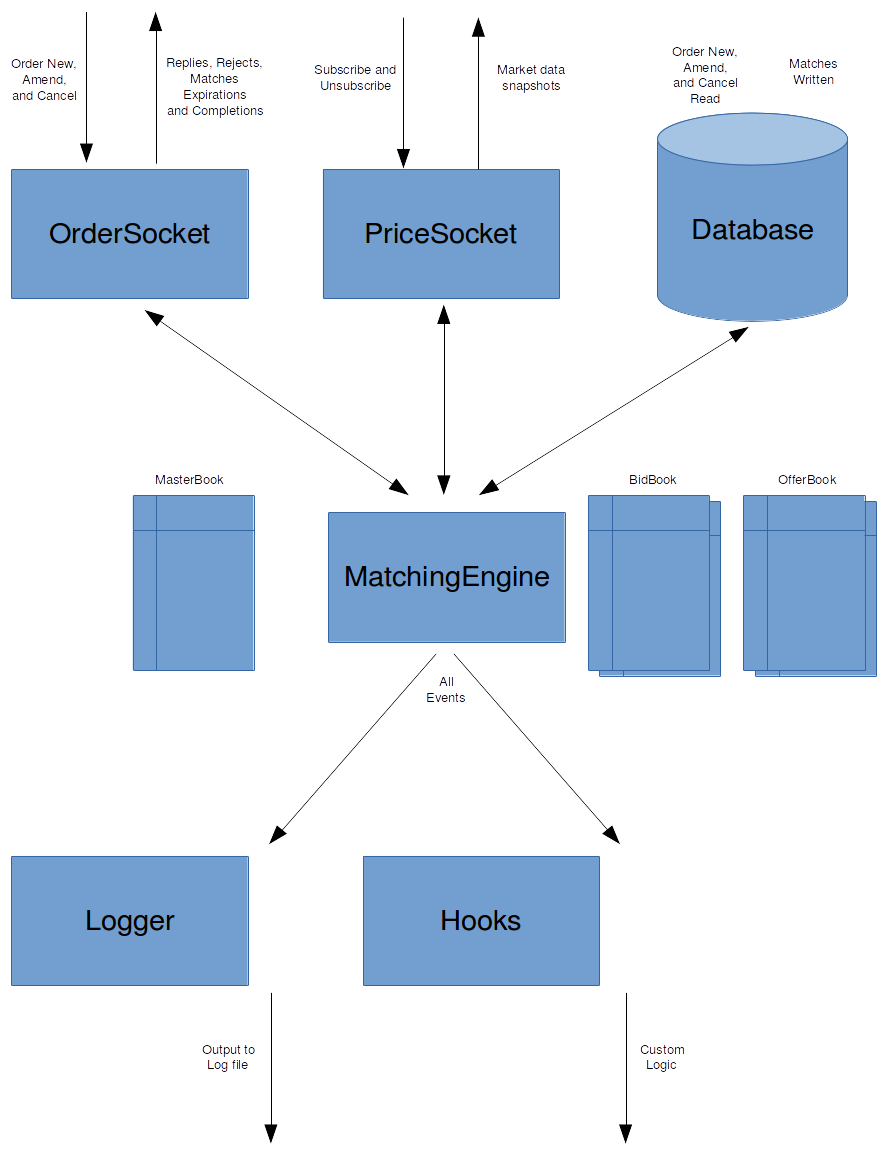
\includegraphics{images/Microssa-Components.png}
\caption{Component Map \label{overflow}}
\end{figure}


\end{document}
